%%=============================================================================
%% Experiment
%%=============================================================================


\chapter{\IfLanguageName{dutch}{Experiment}{Experiment}}
\label{ch:experiment}

\section{Inleiding}
% TODO: move this section to previous chapter
In deze sectie worden de resultaten per benadering opgelijst en besproken. Eerst wordt de benadering kort besproken en worden interessante zaken naar bovengehaald die zich tijdens de implementatie voordeden. Daarna worden de resultaten besproken. Deze resultaten omvatten de aantal lijnen code en de prestaties. \newline \newline Onder de prestatie wordt voornamelijk gekeken naar de CPU-tijd en de overgeslagen frames. De CPU-tijd  is de totaal aantal tijd dat de CPU Dart code heeft uitgevoerd. Dit is een goede benadering voor het batterijverbruik.


\section{ScopedModel}
\subsection{Beschrijving}
% gebruikte packages en hoe was het verloop
De implementatie van de ScopedModel benadering wordt beschouwd als één van de eenvoudigere. De ScopedModel vereist geen drastische wijzigingen in de applicatie structuur. De ontwikkelaar schrijft klasse modellen en laat deze eenvoudig uitbreiden van de \verb|Model| klasse. Zo beschikt de applicatie in deze benadering over een winkel, product en voorkeuren model. \newline
Voor deze benadering wordt enkel beroep gedaan op de \verb|scoped_model| package. 

\subsection{Resultaten}
\subsubsection{Aantal lijnen code}
Deze benadering vereist geen boilerplate code en is eenvoudig te implementeren. Voor deze benadering zijn in totaliteit 802 lijnen code geschreven. Dit reflecteert zich in de aantal lijnen code. In vergelijking met de aantal lijnen code van de boilerplate code, die 711 bedraagt, is dit geen groot verschil. 

Op basis van de aantal lijnen code resulteert de ScopedModel benadering als een toegankelijke benadering die snel is uit te schrijven.

\subsubsection{Prestaties}
Onderstaande tabel \ref{table:experiment-scopedmodel-statistics} beschrijft de CPU-tijd, inclusief enkele statistieken. De CPU-tijd wordt genoteerd in millisecondes. Alle getallen worden indien nodig afgerond op twee cijfers na de komma.
\begin{table}[H]
    \centering
    \begin{tabular}{c|c}
        \textbf{Berekening} & \textbf{CPU-tijd (in ms)} \\ \hline
        Minimum             & 388                       \\ \hline
        Maximum             & 87425                     \\ \hline
        Gemiddelde          & 6770.60                   \\ \hline
        Mediaan             & 4664                      \\ \hline
        Standaardafwijking  & 7426.88                   \\ \hline
        Variantie           & 55158497                  \\ \hline
        Modus               & 1681                      \\                
    \end{tabular}
    \caption{Statistieken van de CPU-tijd bij de ScopedModel benadering}
    \label{table:experiment-scopedmodel-statistics}
\end{table}

% TODO: move this to previous chapter?
Om een duidend overzicht te verkrijgen over de benadering wordt er een extra meeteenheid bekeken. Er is sprake van een overgeslagen frame wanneer de applicatie een frame niet kan tekenen binnen een bepaalde periode. Als gevolg dat de frame wordt overgeslagen. Dit resulteert in de UI die niet vloeiend overkomt. \autocite{Flutter2019d}.

Tijdens het doorlopen van de ScopedModel benadering zijn in totaal 838 frames overgeslagen. Dit komt neer op een gemiddelde van 16.76 overgeslagen frames per uitvoering.

\section{Provider}
\subsection{Beschrijving}
De Provider benadering is gelijkaardig aan die van ScopedModel. Zowel de structuur van de code als de toegankelijkheid is te vergelijken met die van ScopedModel. Het enige verschil is dat de model klassen bij ScopedModel overerven van \verb|ChangeNotifier| in plaats van \verb|Model|. \newline
Voor deze benadering wordt enkel beroep gedaan op de \verb|provider| package. 

\subsection{Resultaten}
\subsubsection{Aantal lijnen code}
Voor deze benadering zijn in totaliteit 804 lijnen code geschreven. Net zoals ScopedModel is deze benadering toegankelijk en snel uit te schrijven.

\subsubsection{Prestaties}
Onderstaande tabel \ref{table:experiment-provider-statistics} beschrijft de CPU-tijd, inclusief enkele statistieken. De CPU-tijd wordt genoteerd in millisecondes. Alle getallen worden indien nodig afgerond op twee cijfers na de komma.
\begin{table}[H]
    \centering
    \begin{tabular}{c|c}
        \textbf{Berekening} & \textbf{CPU-tijd (in ms)} \\ \hline
        Minimum             & 371                       \\ \hline
        Maximum             & 76430                     \\ \hline
        Gemiddelde          & 5410.97                   \\ \hline
        Mediaan             & 3696.50                   \\ \hline
        Standaardafwijking  & 6066.37                   \\ \hline
        Variantie           & 36800785                  \\ \hline
        Modus               & 1410                      \\                
    \end{tabular}
    \caption{Statistieken van de CPU-tijd bij de Provider benadering}
    \label{table:experiment-provider-statistics}
\end{table}

Tijdens het doorlopen van de Provider benadering zijn in totaal 595 frames overgeslagen. Dit komt neer op een gemiddelde van 11.90 overgeslagen frames per uitvoering.

\section{BLoC - RxDart}
\subsection{Beschrijving}
In deze benadering wordt een BLoC gemaakt voor de winkel en de voorkeuren. De architectuur bij deze benadering is anders dan die bij ScopedModel en/of Provider. 
De aanwezigheid van de \verb|BlocProvider| klasse zorgt ervoor dat de geïnjecteerde BLoCs doorheen de applicatie opgevraagd kunnnen worden. 
Volgende code wordt uitgelegd:

\begin{minted}{dart}
class PreferencesBloc extends BlocBase {
    bool _isDarkTheme = false;
    
    final _isDarkThemeController = BehaviorSubject<bool>();
    Stream<bool> get isDarkTheme => _isDarkThemeController.stream;
    
    final _toggleThemeController = BehaviorSubject<void>();
    Sink<void> get toggleTheme => _toggleThemeController.sink;
    
    PreferencesBloc() {
        _isDarkThemeController.add(_isDarkTheme);
    
        _toggleThemeController.listen(_handleToggleTheme);
    }
    
    void _handleToggleTheme(void event) {
        _isDarkTheme = !_isDarkTheme;
    
        _isDarkThemeController.add(_isDarkTheme);
    }
    
    @override
    void dispose() {
        _isDarkThemeController.close();
        _toggleThemeController.close();
    }
}
\end{minted}
In de constructor van de \verb|PreferencesBloc| wordt de initiële waarde van de \verb|isDarkTheme| stream ingesteld. Hier wordt ook de luisteraar toegevoegd aan de \verb|_toggleThemeController|. Deze \verb|_handleToggleTheme| methode zal de nodige business logica afhandelen en zodanig een nieuw event toevoegen aan de \verb|isDarkTheme| stream.
De abstracte \verb|BlocBase| klasse bevat enkel een verplichte te implementeren \verb|dispose()| methode. In deze methode worden de streams gesloten. \newline
Voor deze benadering wordt enkel beroep gedaan op de \verb|rxdart| package. 

\subsection{Resultaten}
\subsubsection{Aantal lijnen code}
Voor deze benadering zijn in totaliteit 927 lijnen code geschreven. Vergeleken met vorige benaderingen is dit direct al pak meer. In vergelijking met ScopedModel en Provider is dit om en beide 15\% meer code. Indien een applicatie een zodanige grote heeft is dit wel een gevolg om in acht te nemen. Dit reflecteert evenredig met de complexiteit. De BLoC benadering vraagt een andere manier van denken voor de ontwikkelaar. De vraag is of de ontwikkelaar de nodige tijd wil investeren om deze bendaring onder de knie te krijgen. Dit is een vraagstuk waar alleen de ontwikkelaar zelf een antwoord kan op bieden.

Het valt in overweging te nemen of de ontwikkelaar een gestructureerdere aanpak wil hanteren met als neveneffect meer code. Merk op dat indien een gestructureerdere aanpak wordt gehanteerd dit kan resulteren in een gemakkelijker in de toekomst. 
\subsubsection{Prestaties}
Onderstaande tabel \ref{table:experiment-bloc-rxdart-statistics} beschrijft de CPU-tijd, inclusief enkele statistieken. De CPU-tijd wordt genoteerd in millisecondes. Alle getallen worden indien nodig afgerond op twee cijfers na de komma.
\begin{table}[H]
    \centering
    \begin{tabular}{c|c}
        \textbf{Berekening} & \textbf{CPU-tijd (in ms)} \\ \hline
        Minimum             & 366                       \\ \hline
        Maximum             & 69670                     \\ \hline
        Gemiddelde          & 5556.28                   \\ \hline
        Mediaan             & 3861                      \\ \hline
        Standaardafwijking  & 5913.87                   \\ \hline
        Variantie           & 34973841                  \\ \hline
        Modus               & 3280                      \\                
    \end{tabular}
    \caption{Statistieken van de CPU-tijd bij de BLoC-RxDart benadering}
    \label{table:experiment-bloc-rxdart-statistics}
\end{table}

Tijdens het doorlopen van de BLoC - RxDart benadering zijn in totaal 610 frames overgeslagen. Dit komt neer op een gemiddelde van 12.20 overgeslagen frames per uitvoering.

\section{Redux}
\subsection{Beschrijving}
Van alle benaderingen vergt Redux de grootste wijziging in de manier van denken. De leercurve van Redux is immers stukken groter vergeleken met de andere benaderingen. Opnieuw komt hier hetzelfde argument als bij BLoC terug: in hoeverre wenst de ontwikkelaar tijd te investeren om een State Management onder de knie te krijgen. Eenmaal het concept van Redux duidelijk is, is het gemakkelijk om een applicatie uit te breiden. 
Als de Redux benadering wordt vergeleken met die van bijvoorbeeld Provider zijn er geen gelijkenissen. De architectuur van de applicatie is verschillend op heel wat vlakken, dit mede dankzij de concepten van Redux. \newline
Voor deze benadering wordt beroep gedaan op volgende packages: 
\begin{itemize}
    \item{redux}
    \item{flutter\_redux}
\end{itemize}
\subsection{Resultaten}


\subsubsection{Aantal lijnen code}
Voor deze benadering zijn in totaliteit 1042 lijnen code geschreven. In vergelijking met ScopedModel of Provider is dit 22\% meer code. Vergeleken met de BLoC is dit afgerond 11\%. \newline
De oorzaak van de hoeveelheid aantal lijnen code is te danken aan de boilerplate code die geschreven moet worden bij Redux. Er worden actions, reducers opgesteld, dit zorgt voor de vele aantal lijnen code. De voorkeuren en winkel state wordt dan nog eens globaal ingewikkeld in de zogenaamde app state die gebruikt wordt doorheen de applicatie.

\subsubsection{Prestaties}
Onderstaande tabel \ref{table:experiment-redux-statistics} beschrijft de CPU-tijd, inclusief enkele statistieken. De CPU-tijd wordt genoteerd in millisecondes. Alle getallen worden indien nodig afgerond op twee cijfers na de komma.
\begin{table}[H]
    \centering
    \begin{tabular}{c|c}
        \textbf{Berekening} & \textbf{CPU-tijd (in ms)} \\ \hline
        Minimum             & 376                       \\ \hline
        Maximum             & 78013                     \\ \hline
        Gemiddelde          & 6435.20                   \\ \hline
        Mediaan             & 4264                      \\ \hline
        Standaardafwijking  & 7420.15                   \\ \hline
        Variantie           & 55058683                  \\ \hline
        Modus               & 3964                      \\                
    \end{tabular}
    \caption{Statistieken van de CPU-tijd bij de Redux benadering}
    \label{table:experiment-redux-statistics}
\end{table}

Tijdens het doorlopen van de Redux benadering zijn in totaal 820 frames overgeslagen. Dit komt neer op een gemiddelde van 16.73 overgeslagen frames per uitvoering.

\section{MobX}
\subsection{Beschrijving}

Voor deze benadering wordt beroep gedaan op volgende packages: 
\begin{itemize}
    \item{mobx}
    \item{flutter\_mobx}
    \item{provider}
\end{itemize}
Opmerking de \verb|provider| package wordt hier enkel en alleen gebruikt als oplossing voor dependency injection.

\subsection{Resultaten}
\subsubsection{Aantal lijnen code}
Voor deze benadering zijn in totaliteit 928 lijnen code geschreven.
\subsubsection{Prestaties}
Onderstaande tabel \ref{table:experiment-mobx-statistics} beschrijft de CPU-tijd, inclusief enkele statistieken. De CPU-tijd wordt genoteerd in millisecondes. Alle getallen worden indien nodig afgerond op twee cijfers na de komma.
\begin{table}[H]
    \centering
    \begin{tabular}{c|c}
        \textbf{Berekening} & \textbf{CPU-tijd (in ms)} \\ \hline
        Minimum             & 390                       \\ \hline
        Maximum             & 68405                     \\ \hline
        Gemiddelde          & 5498.88                   \\ \hline
        Mediaan             & 3801                      \\ \hline
        Standaardafwijking  & 6128.42                   \\ \hline
        Variantie           & 37557505                  \\ \hline
        Modus               & 2544                      \\                
    \end{tabular}
    \caption{Statistieken van de CPU-tijd bij de MobX benadering}
    \label{table:experiment-mobx-statistics}
\end{table}

Tijdens het doorlopen van de MobX benadering zijn er in totaliteit 572 frames overgeslagen. Dit komt neer op een gemiddelde van 11.40 overgeslagen frames per uitvoering.

\section{Samenvatting}

In onderstaande tabel \ref{table:amount-lines-of-code} worden de aantal lijnen code per benadering opgesomd. De rij ``gecorrigeerd'' is het aantal lijnen code van de benadering min het aantal lijnen code van de boilerplate code.
\begin{table}[H]
    \centering
    \begin{tabular}{c|c|c|c|c|c}
        & \textbf{ScopedModel} & \textbf{Provider} & \textbf{BLoC} & \textbf{Redux} & \textbf{MobX} \\ \hline
        Totaal               & 802   &  804     &  927     &  1042    &  928        \\ \hline
        Gecorrigeerd         & 91    &  93      &  216     &  331     &  217
    \end{tabular}
    \caption{Statistieken van het aantal lijnen code van alle benaderningen}
    \label{table:amount-lines-of-code}
\end{table}

\begin{table}[H]
    \centering
    \begin{tabular}{c|c|c|c|c|c}
        & \textbf{ScopedModel} & \textbf{Provider} & \textbf{BLoC} & \textbf{Redux} & \textbf{MobX} \\ \hline
        Minimum             & 388        &  371        &  366       &  376       &  390        \\ \hline
        Maximum             & 87425      &  76430      &  69670     &  78013     &  68405      \\ \hline
        Gemiddelde          & 6770.60    &  5410.97    &  5556.28   &  6435.20   &  5498.88    \\ \hline
        Mediaan             & 4664       &  3696.50    &  3861      &  4264      &  3801       \\ \hline
        Standaardafwijking  & 7426.88    &  6066.37    &  5913.87   &  7420.15   &  6128.42    \\ \hline
        Variantie           & 55158497   &  36800785   &  34973841  &  55058683  &  37557505   \\ \hline
        Modus               & 1681       &  1410       &  3280      &  3964      &  2544       \\                
    \end{tabular}
    \caption{Statistieken van de CPU-tijd (in ms) van alle benaderningen}
    \label{table:experiment-cpu-time}
\end{table}

\begin{table}[H]
    \centering
    \begin{tabular}{c|c|c|c|c|c}
        & \textbf{ScopedModel} & \textbf{Provider} & \textbf{BLoC} & \textbf{Redux} & \textbf{MobX} \\ \hline
        Totaal      &  838   &  595     &  610     &  820    &  572        \\ \hline
        Gemiddeld   &  16.76    &  11.90   &  12.20   &  16.73  &  11.40        \\ 
    \end{tabular}
    \caption{Statistieken van de totaal en gemiddeld aantal overgeslagen frames van alle benaderingen}
    \label{table:experiment-skipped-frames}
\end{table}

\begin{figure}[H]
    \centering
    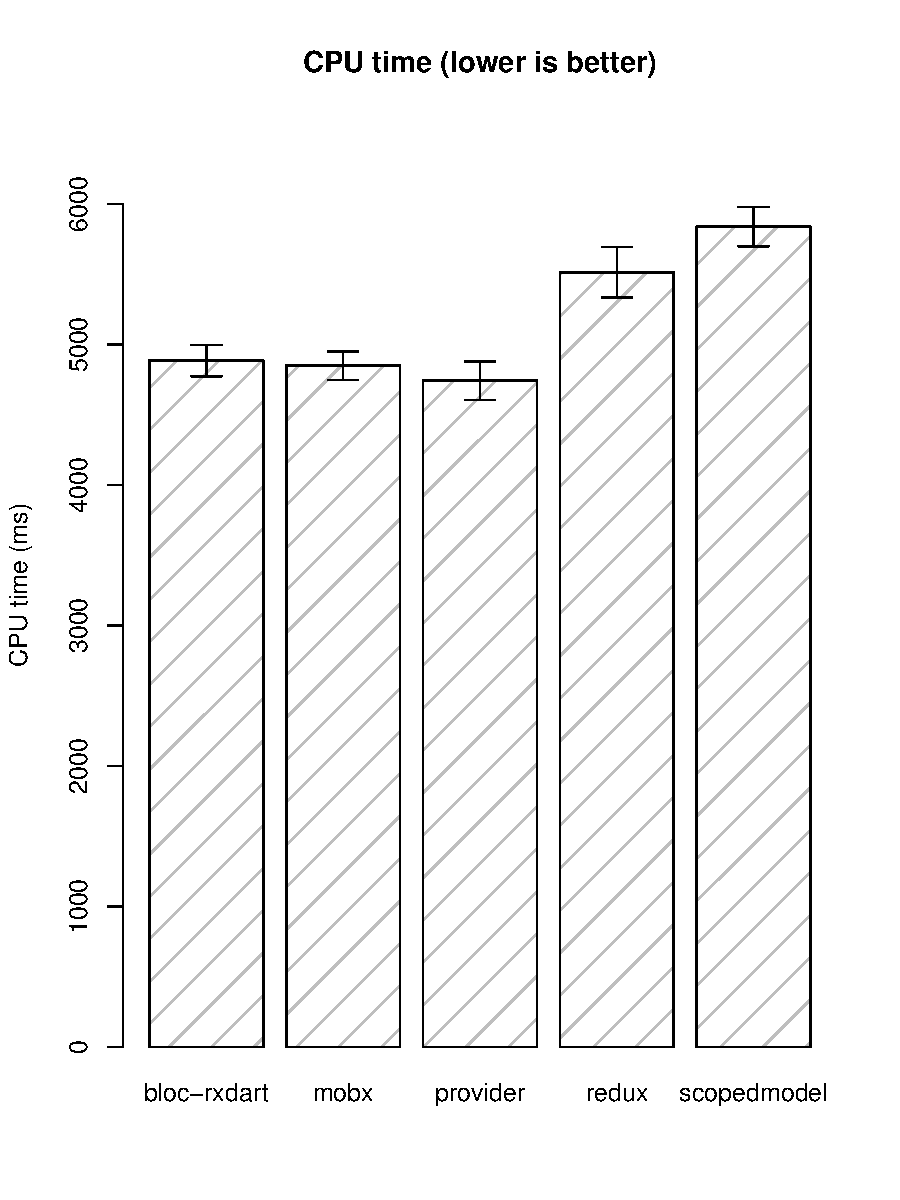
\includegraphics[width=\linewidth]{img/experiment/cpu_time.pdf}
    \caption{Grafiek van de CPU-tijd van de verschillende benaderingen}
    \label{fig:graph-cpu-time}
\end{figure}
% al de grafieken samen? Tabel?